\section{Theory} \label{sec:Theory}

The fundamental parts of the predictive model are the conservation of particles (\cref{sub:ParticleConservation}), momentum (\cref{sub:MomentumConservation}), and energy (\cref{sub:EnergyConservation}), the conduction closure (\cref{sub:ConductionClosure}) and the ideal gas law (\cref{sub:IdealGasLaw}). Within each of the conservation equations there is provision for the removal of particles, momentum, and energy due to \ac{IOL}, which is described in \cref{sub:IOL}. \ac{IOL} calculation requires input from the equilibrium reconstruction. Therefore, a short overview is provided in \cref{subsub:EFIT}.  The primary source of particles, momentum, and energy considered is beam input and therefore, details on the beam modeling are covered in \cref{sub:BeamModeling}. Finally, the pinch diffusion model is described, because there is a desire to recast the conservation equations in the form of a pinch diffusion equation. Therefore, the pinch diffusion model will be discussed in \cref{sub:PinchDiffusion}

\subsection{Conservation of Particles} \label{sub:ParticleConservation}

The general multidimensional form of the continuity equation in \cref{eqn:GeneralContinuity}
%
\begin{equation}
	\symbf{\nabla} \cdot n_j \symbf{v}_j = S_j
	\label{eqn:GeneralContinuity}
\end{equation}
%
reduces to the one-dimensional non-linear \ac{ODE} shown in \cref{eqn:Continuity} and \cref{eqn:Source} when one performs a \ac{FSA}. The reason is that the poloidal component of the flux, $\langle \left(\symbf{\nabla} \cdot n_j \symbf{v}_j \right)_\theta \rangle = 0$ identically and $\langle \left(\symbf{\nabla} \cdot n_j \symbf{v}_j \right)_\phi \rangle = 0$ by axisymmetry \cite{Stacey2004}.

\begin{equation}
	\cfrac{1}{r} \diffpfunc{ r \func{\Gamma_{rj}}{r}}{r} =
	S_{nj} -\alpha \diffpfunc{ \FrIOL{j} }{r} \flux{j}
	-\beta z_{k} \diffpfunc{ \FrIOL{k} }{r} \flux{k}
	\label{eqn:Continuity}
\end{equation}
%
where,
%
\begin{equation}
	S_{nj} \equiv \func{N_\mathrm{nbj}}{r} \left( 1\ -\hat{\alpha } \func{f^\mathrm{iol}_\mathrm{nbi}}{r} \right)+ \func{n_{e}}{r} \nu _{\mathrm{ion}_j} (r)
	\label{eqn:Source}
\end{equation}

The left side of \cref{eqn:Continuity} expresses the change in flux, $\Gamma_{rj}$ of the primary ion is driven by the source terms on the right. First, $S_{nj}$, is the positive contributions due to \ac{NBI} and ionization. In \cref{eqn:Source}, $N_{nbj}$ is the rate of \ac{NBI} injection, which has been reduced by the fast \ac{IOL}, $f^\mathrm{iol}_\mathrm{nbi}$. The rate of neutral beam injection is based on a beam model that is described in \cref{sub:BeamModeling}. The second term, $\func{n_{e}}{r} \nu _{\mathrm{ion}_j} (r)$ is the ionization rate and is discussed in \cref{sub:NeutralTransport}. Lastly, in \cref{eqn:Continuity}, there are two terms for \ac{IOL}, $\FrIOL{j}$ for the primary ion, and $\FrIOL{k}$ for the impurity ion. They are the cumulative loss of ions through the mechanism of \ac{IOL}. They impact the conservation of particles through their differential contributions, $\diffp{}{r}$. These \ac{IOL} terms are detailed in \cref{sub:IOL}. The terms, $\alpha$ and $\beta$ are charge neutrality adjustment terms and will be a subject of consideration. There are three mechanisms by which the charge associated with lost primary ions can be compensated:

\begin{enumerate}[label=(\roman*)]
	\item A commensurate lost electrons implying $\left(\alpha=1, \beta=0\right)$ thus nullifying $\FrIOL{k}$, \label{item:NeutElectron}
	\item A return current of thermalized ions from the \ac{SOL} (\gls{SOL}) implying $\left(\alpha=2, \beta=1\right)$, or \label{item:NeutImpurity}
	\item No \ac{IOL} $\left(\alpha=0, \beta=0\right)$ \label{item:NeutNoIOL}
\end{enumerate}

\citeauthor{Stacey2017} conjectures that the most physically reasonable is \cref{item:NeutImpurity}, which we intend to explore.


%\symdef{$r$}{Location along the minor radius}{\emath{L}}{$m$}
%\nomenclature{$\hat{\Gamma}_{rj}$}{Radial flux for primary ion j}{L}{dum}
%\nomenclature{$S_n$}{Particle source}
%\nomenclature{$F^{IOL}$}{Thermal Ion Orbit Loss fraction}
%\nomenclature{$\alpha, \beta$}{Charge neutrality adjustment term}
%\nomenclature{$f^{IOL}$}{Fast Ion Orbit Loss fraction}
%\nomenclature{$z$}{Atomic Number}
%\nomenclature{$N_{nb}$}{Fast Neutral Beam Source Rate}
%\nomenclature{$\hat{\alpha}$}{description}
%\nomenclature{$\nu_{ion}$}{Frequency of Ionization}
%\nomenclature{$n$}{Species number density}
%\nomenclature{$L_p^{-1}$}{Pressure Gradient Scale Length $\frac{1}{p} \diffp{p}{r}$ }
%\nomenclature{$L_T^{-1}$}{Temperature Gradient Scale Length $\frac{1}{T} \diffp{T}{r}$ }

%\subsection{Ion Orbit Loss} \label{sub:IOL}

\acf{IOL} represents a non-diffusive mechanism for losing particles. At the heart of \ac{IOL} theory is an electromagnetic equilibrium argument that, to a first order, between any two flux surfaces canonical angular momentum (\cref{eqn:IOLCanonAngleMom}), energy (\cref{eqn:IOLEnergy}), and magnetic moment (\cref{eqn:IOLMagMom}) are conserved. Based on this fundamental principle, \citeauthor{Miyamoto1996} \cite{Miyamoto1996} observed that one could use the values of plasma parameters on an inner flux surface (marked with a subscript 0) and the parameters on a separatrix, (marked with a subscript s or no subscript). \prettyref{fig:featuressofatokamakplasma} illustrates two flux surfaces, one being the separatrix and an inner one between the core and edge region.

\begin{equation}
	\left[ R\, m\, V_\parallel \left(\cfrac{B_\varphi}{B}\right) + e \psi \right]_0
	=
	\left[ R\, m\, V_\parallel \left(\cfrac{B_\varphi}{B}\right) + e \psi \right]_s 
	\label{eqn:IOLCanonAngleMom}
\end{equation}

\begin{equation}
	\left[ \cfrac{1}{2} \left( V_\parallel^2 + V_\perp^2  \phantom{\cfrac{1}{2}}\right) \right]_0
	=
	\left[ \cfrac{1}{2} \left( V_\parallel^2 + V_\perp^2  \phantom{\cfrac{1}{2}}\right) \right]_s
	\label{eqn:IOLEnergy}	
\end{equation}

\begin{equation}
	\left[ \cfrac{m\,V_\perp^2}{2\,B} \right]_0
	=
	\left[ \cfrac{m\,V_\perp^2}{2\,B} \right]_s
	\label{eqn:IOLMagMom}
\end{equation}

Utilizing \cref{eqn:IOLV0}, defining the term $f_\varphi$ in \cref{eqn:IOLfphi} and the parameter $\zeta_0$, which is the direction cosine of the particles launch angle with respect to the toroidal magnetic field line, $B_\varphi$, \crefrange{eqn:IOLCanonAngleMom}{eqn:IOLMagMom} can be rewritten into \cref{eqn:IOLMinV0}. This equation, which is quadratic in $V_0$, represents the equilibrium velocity for a particle to have an orbit that is within the confined portion of the plasma, meaning within the separatrix.

\begin{equation}
	V_0 = \sqrt{V_\parallel^2 + V_\perp^2}
	\label{eqn:IOLV0}
\end{equation}

\begin{equation}
	f_\varphi = \left|\cfrac{B_\varphi}{B}\right|
	\label{eqn:IOLfphi}
\end{equation}

\begin{equation}
	\zeta_0 = \cfrac{V_{\parallel 0}}{V_0}
	\label{eqn:IOLzeta0}
\end{equation}

This then serves as the criterion for which a particle can be lost. If it has an energy in excess of this, then it will have an orbit outside of the confined plasma and can encounter a variety of obstructions, such as magnetic field imperfections, \ac{SOL} particles, and most obviously, the wall. The manner by which this minimum velocity is applied to calculate a loss estimate is described in \cref{subsub:CumulativeLoss}.

\begin{equation}
	\begin{gathered}
			V^2_0 \left[ \left( \cfrac{R_0}{R} \cfrac{f_{\varphi 0}}{f_{\varphi}} \zeta_0 \right)^2 -1 + 
		\left( 1 - \zeta^2_0 \right) \left| \cfrac{B}{B_0} \right|  \right] + 
		V_0 \left[ \cfrac{2e \left( \psi_0 - \psi \right) }{R m f_\varphi} \left( \cfrac{R_0}{R}  \cfrac{f_{\varphi 0}}{f_\varphi} \zeta_0 \right)^{\vphantom{2}}   \right] \\
		+ \left[ \left( \cfrac{e\left( \psi_0 - \psi \right) }{R m f_\varphi} \right)^2 - \cfrac{2 e \left(\phi_0 - \phi  \right) }{m} \right] = 0
	\end{gathered}
	\label{eqn:IOLMinV0}
\end{equation}

\prettyref{fig:iolCalc} shows the minimum energy calculations against plasma ion temperature, what this illustrates is that \ac{IOL} is not a dominant transport mechanism for the plasma core. However, it becomes the dominant effect in the last 5\% \cite{Stacey2013} and drives the features in this region.

\begin{figure}
	\centering
	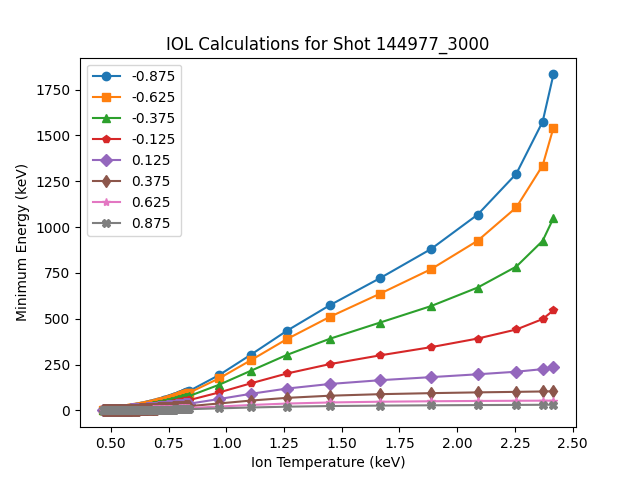
\includegraphics[width=0.5\linewidth]{images/iol_calculations}
	\caption[IOL Calculation]{Minimum Energy calculation for Shot 144977.3000}
	\label{fig:iolCalc}
\end{figure}


\subsubsection{Cumulative Loss Fraction} \label{subsub:CumulativeLoss}

The temperature of any flux surface is assumed to be Maxwellian in the velocity space, which means that if one assumes a three dimensional velocity space, the distribution of energy is given by a Gamma distribution as illustrated in \prettyref{fig:maxwellianGeneral}. The cumulative loss fraction, $F_{rj}^{IOL}$, is determined by truncating the distribution above the minimum energy given in \cref{eqn:IOLEmin}. This leads to an evaluation of the incomplete Gamma distribution, $\BbbGamma$, at $\epsilon\left(\rho,\zeta_0\right)$. The zeroth moment, which corresponds to particle loss, results in a $\BbbGamma\left(\frac{3}{2}\right)$ shown in \cref{eqn:IOLCumulativeLossParticle}. The first moment, which corresponds to momentum loss, results in $\BbbGamma\left(2\right)$ shown in \cref{eqn:IOLCumulativeLossMomentum}. The second moment, which corresponds to energy loss, results in $\BbbGamma\left(\frac{5}{2}\right)$ shown in \cref{eqn:IOLCumulativeLossEnergy}.

\begin{equation}
	\epsilon_{min} = \cfrac{1}{2} m \, V_0^2
	\label{eqn:IOLEmin}
\end{equation}

\begin{figure}[!hb]
	\subfloat[Core Region] {
		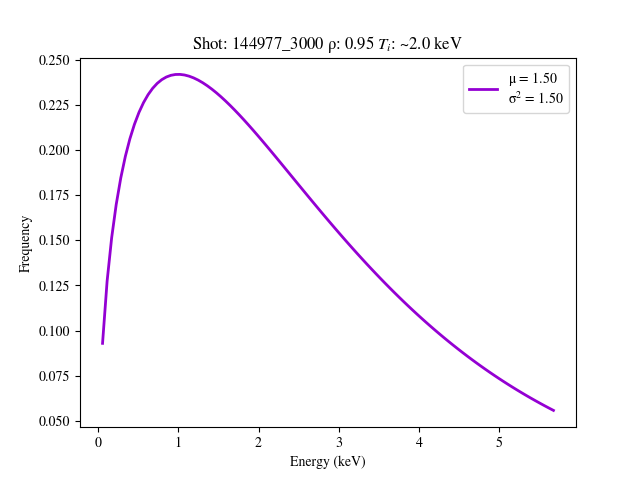
\includegraphics[width=0.5\linewidth]{images/maxwellian_illustration}
		\label{fig:maxwellianGeneral}
	} \quad
	\subfloat[$\rho=0.98$, $T_i=0.517 keV$] {
		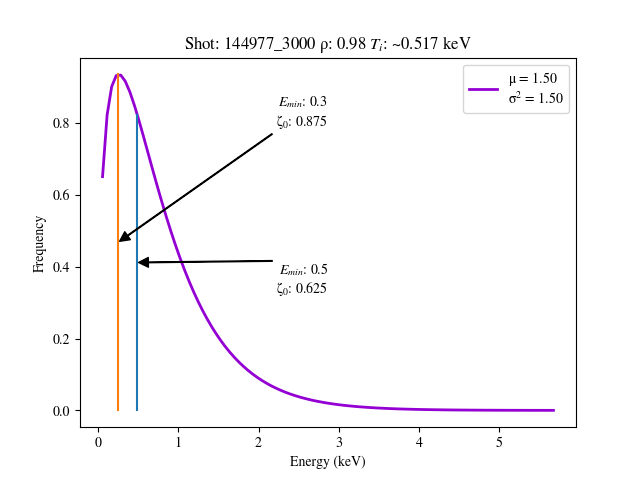
\includegraphics[width=0.5\linewidth]{images/maxwellian_illustration_144977_3000_rho976}
		\label{fig:maxwellianEdge}
	}
	\caption{Maxwellian Gamma Distribution for shot 144977.3000}
\end{figure}

One aspect of the \ac{IOL} that is important to note is that the equilibrium given by \crefrange{eqn:IOLCanonAngleMom}{eqn:IOLMagMom} identify which particles have energy that take them beyond the \ac{LCFS}, but this does not necessarily imply loss. Instead it implies a sufficient orbit to enter unfavorable zones. From this observation, one has to postulate that a certain number of these particles will either i) suffer a collision in the \ac{SOL}, which is not collisionless and therefore reasonable, or ii) particles strike the wall. With this in mind, we utilize the Stacey rational approximation that $R_{loss}^{IOL}$ is approximately 0.5, the logic being that some is more likely than none, while all is probably too much. Half is about right.

\begin{equation}
	F_{rj}^{IOL} \left( r \right) = \cfrac{N_{loss}}{N_{total}} = \cfrac{R_{loss}^{IOL} \bigints_{-1}^{1} \left[ \bigintss_{V_{0,min}}^{\infty} V_0^2 f\left( V_0 \right) dV_0\right] d \zeta_0}{2 \bigintss_{0}^{\infty} V_0^2 f\left(V_0\right)dV_0} = 
	\cfrac{R_{loss}^{IOL} \bigints_{-1}^{1} \BbbGamma \left(\cfrac{3}{2}, \epsilon_{min}\left(\rho,\zeta_0\right)   \right) d\zeta_0}{2 \BbbGamma \left(\cfrac{3}{2}\right)}
	\label{eqn:IOLCumulativeLossParticle}
\end{equation}

\begin{equation}
	M_{rj}^{IOL} \left( r \right) = \cfrac{M_{loss}}{M_{total}} = 
	\cfrac{R_{loss}^{IOL} \bigints_{-1}^{1} \left[ \bigintss_{V_{0,min}}^{\infty} 
		\left(m\,V_0\,\zeta_0\right) V_0^2 f\left( V_0 \right) dV_0\right] d\zeta_0}{2 \bigintss_{0}^{\infty} \left(m\,V_0\right) V_0^2 f\left(V_0\right)dV_0} = 
	\cfrac{R_{loss}^{IOL} \bigints_{-1}^{1} \BbbGamma \left(2, \epsilon_{min}\left(\rho,\zeta_0\right)   \right) d\zeta_0}{2 \BbbGamma \left(2\right)}
	\label{eqn:IOLCumulativeLossMomentum}
\end{equation}


\begin{equation}
	E_{rj}^{IOL} \left( r \right) = \cfrac{E_{loss}}{E_{total}} = \cfrac{R_{loss}^{IOL} \bigints_{-1}^{1} \left[ \bigintss_{V_{0,min}}^{\infty} \left(\cfrac{1}{2} m\,V_0^2\right) V_0^2 f\left( V_0 \right) dV_0\right] d\zeta_0}{2 \bigintss_{0}^{\infty} \left(\cfrac{1}{2} m\,V_0^2\,\zeta_0\right) V_0^2 f\left(V_0\right)dV_0} = 
	\cfrac{R_{loss}^{IOL} \bigints_{-1}^{1} \BbbGamma \left(\cfrac{5}{2}, \epsilon_{min}\left(\rho,\zeta_0\right)   \right) d\zeta_0}{2 \BbbGamma \left(\cfrac{5}{2}\right)} 
	\label{eqn:IOLCumulativeLossEnergy}
\end{equation}


%
%\subsection{Conservation of Momentum} \label{sub:MomentumConservation}

A very important aspect of the equations utilized for this research is that the momentum conservation recovers the fundamental electromagnetic principle inherent in the Lorentz \vxb forces, which are orthogonal to the direction of motion. 
%
\begin{equation}
	\vec{F} = e(\vec{E} + \vxb)
	\label{eqn:Lorentz}
\end{equation}
%
For this reason the bulk fluid toroidal, $V_\varphi$, and poloidal $V_\theta$ velocities influence the radial momentum conservation in \cref{subsub:MCRadial} and the poloidal in \cref{subsub:MCPoloidal}. Additionally, because there is a radial particle flux outward, $\Gamma_{rj},\Gamma_{rk}$, there is a radial electric field that manifests.

\subsubsection{Radial} \label{subsub:MCRadial}
The radial momentum equates the normal force of pressure gradient with the orthogonal contribution of the \vxb. A technique to recapture the pressure is to utilize the gradient scale length (\cref{eqn:GradScalePressure}). It is an empirically derived parameter that is determined from a form of the equations that we are solving \cite{Stacey2004a} and represents a fundamental property in the plasma edge. In the radial direction, the \vxb terms that contribute to the force balance are the $e V_\theta \, B_\varphi$ and the $e$

\begin{equation}
	L_p^{-1} \equiv = \cfrac{1}{p} \diffp{p}r
	\label{eqn:GradScalePressure}
\end{equation}

\begin{equation}
	\begin{bmatrix}
		p_j L^{-1}_{p_j} \\
		p_k L^{-1}_{p_k}
	\end{bmatrix} =
	\begin{bmatrix}
		-\cfrac{1}{1+\cfrac{z_j}{z_k} \cfrac{n_j}{n_k}} & \cfrac{1}{1+\cfrac{z_k}{z_j} \cfrac{n_k}{n_j}} \\
		\cfrac{1}{1+\cfrac{z_k}{z_k} \cfrac{n_j}{n_k}} & -\cfrac{1}{\cfrac{n_k}{n_j} \cfrac{z_k}{z_j}+1}
	\end{bmatrix}^{-1} 
	\begin{bmatrix}
		\cfrac{n_j z_j}{1+\cfrac{n_j}{n_k} \cfrac{m_j}{m_k}} & \cfrac{n_j z_j}{1+\cfrac{n_j}{n_k} \cfrac{m_j}{m_k}} \\
		\cfrac{n_k z_k}{1+\cfrac{n_k}{n_j} \cfrac{m_k}{m_j}} & \cfrac{n_j z_j}{1+\cfrac{n_k}{n_j} \cfrac{m_k}{m_j}}
	\end{bmatrix} 
	\begin{bmatrix}
		e B_\varphi
		\begin{bmatrix}
			V_{\theta j} \\
			V_{\theta k}
		\end{bmatrix} -
		e B_\theta
		\begin{bmatrix}
			V_{\varphi j} \\
			V_{\varphi k}
		\end{bmatrix}
	\end{bmatrix}
	\label{eqn:ConservationOfMomentumRadial}
\end{equation} 


%\begin{multline}
%	\begin{bmatrix}
%		-\cfrac{1}{1+\cfrac{z_j}{z_k} \cfrac{n_j}{n_k}} & \cfrac{1}{1+\cfrac{z_k}{z_j} \cfrac{n_k}{n_j}} \\
%		\cfrac{1}{1+\cfrac{z_k}{z_k} \cfrac{n_j}{n_k}} & -\cfrac{1}{\cfrac{n_k}{n_j} \cfrac{z_k}{z_j}+1}
%	\end{bmatrix} 
%	\begin{bmatrix}
%		p_j L^{-1}_{p_j} \\
%		p_k L^{-1}_{p_k}
%	\end{bmatrix} = \\		
%	\begin{bmatrix}
%		\cfrac{n_j e z_j}{1+\cfrac{n_j}{n_k} \cfrac{m_j}{m_k}} & \cfrac{n_j e z_j}{1+\cfrac{n_j}{n_k} \cfrac{m_j}{m_k}} \\
%		\cfrac{n_k e z_k}{1+\cfrac{n_k}{n_j} \cfrac{m_k}{m_j}} & \cfrac{n_j e z_j}{1+\cfrac{n_k}{n_j} \cfrac{m_k}{m_j}}
%	\end{bmatrix} 
%	B_\phi 
%	\begin{bmatrix}
%		\hat{V}_{\theta_j} \\
%		\hat{V}_{\theta_k}
%	\end{bmatrix} -
%	\begin{bmatrix}
%		\cfrac{n_j e z_j}{1+\cfrac{n_j}{n_k} \cfrac{m_j}{m_k}} & \cfrac{n_j e z_j}{1+\cfrac{n_j}{n_k} \cfrac{m_j}{m_k}} \\
%		\cfrac{n_k e z_k}{1+\cfrac{n_k}{n_j} \cfrac{m_k}{m_j}} & \cfrac{n_j e z_j}{1+\cfrac{n_k}{n_j} \cfrac{m_k}{m_j}}
%	\end{bmatrix} 
%	B_\theta 
%	\begin{bmatrix}
%		\hat{V}_{\phi_j} \\
%		\hat{V}_{\phi_k}
%	\end{bmatrix}
%\end{multline} \label{eqn:ConservationOfMomentumRadial}
\subsubsection{Toroidal} \label{subsub:MCToroidal}

The toroidal momentum balance expressed in \cref{eqn:ConservationMomentumToroidal} equates the forces due to the fluid velocity, $V_\varphi$, with the force due to the toroidal electric field, $E_\varphi^A$, the Lorentz force associated with a radial flux, the momentum input of \ac{NBI} and finally the momentum loss due to \ac{IOL}. It is of some value to deconstruct several of the terms to gain an intuition for these terms.
\begin{itemize}
	\item The force associated with the fluid velocity arises from two physical considerations, collisional drag within the species expressed as a frequency, $\nu_{dj}$, and inter-species drag, $\nu_{jk}$. As an aside it helped the author to do a units analysis that this works to force per unit volume.
	\item The electric field $E_\varphi^A$ is simply a result of current drive and is therefore an externally applied condition.
	\item the $e\,B_\theta \Gamma$ term is a masked Lorentz force. The flux is motion of the charged ionized particles, which produce an orthogonal force as they move across a magnetic field line.
	\item The momentum of the \ac{IOL} term is due to an instantaneous loss of particles. The model description is given in \cref{eqn:IOLCumulativeLossMomentum}
\end{itemize}

\begin{multline}  \label{eqn:ConservationMomentumToroidal}
	\begin{bmatrix}
		n_j m_j \left( \nu_{jk} + \nu^{\varphi}_{dj} \right) & -n_j m_j \nu_{jk} \\
		-n_k m_k \nu_{kj}  & n_k m_k \left( \nu_{kj}+\nu^{\varphi}_{dk} \right)
	\end{bmatrix}
	\begin{bmatrix}
		\hat{V}_{\varphi j}\left(r\right) \\
		\hat{V}_{\varphi k}\left(r\right)								
	\end{bmatrix} = \\
	\begin{bmatrix}
		n_j e_j \\
		n_k e_k
	\end{bmatrix} E^A_{\varphi} +
	\begin{bmatrix}
		e_j B_\theta & 0 \\
		0            & e_k B_\theta
	\end{bmatrix}
	\begin{bmatrix}
		\Gamma_{rj} \left(r\right) \\
		\Gamma_{rk} \left(r\right)
	\end{bmatrix} +
	\begin{bmatrix}
		M_{\varphi j}^\mathrm{nbi}\left(r\right) \\
		M_{\varphi k}^\mathrm{nbi}\left(r\right)
	\end{bmatrix} -
	\begin{bmatrix}
		M_{\varphi j}^\mathrm{iol}\left(r\right) \\
		M_{\varphi k}^\mathrm{iol}\left(r\right)
	\end{bmatrix}
\end{multline}
\subsubsection{Poloidal} \label{subsub:MCPoloidal}

The poloidal momentum conservation is described by \cref{eqn:ConservationOfMomentumPoloidal}. Most of the terms in the poloidal momentum balance are the same as the toroidal momentum balance, which is explained in \cref{subsub:MCToroidal}, but the appropriate changes for the orthogonal Lorentz contributions. The third time on the right of \cref{eqn:ConservationOfMomentumPoloidal}, however, is unique. It results from the gyro-viscous considerations that are negligible in a straight cylindrical plasma, as modeled by Braginskii[\cite{Braginskii1965}], but are significant in a toroidally confined plasma, due to the curvature of the field lines \cite{Stacey2020}. The coefficient, $K$, is the Stacey-Sigmar coefficients which can be found in \citetitle{StaceySigmar1985} \cite{StaceySigmar1985}.

\begin{multline} \label{eqn:ConservationOfMomentumPoloidal}
	\begin{bmatrix}
		n_j m_j \left( \nu_{jk} + \nu^{\theta}_{dj} \right) & -n_j m_j \nu_{jk} \\
		-n_k m_k \nu_{kj}  & n_k m_k \left( \nu_{kj}+\nu^{\theta}_{dk} \right)
	\end{bmatrix}
	\begin{bmatrix}
		\hat{V}_{\theta j}\left(r\right) \\
		\hat{V}_{\theta k}\left(r\right)								
	\end{bmatrix} =
	\begin{bmatrix}
		n_j e_j \\
		n_k e_k
	\end{bmatrix} E^A_{\theta} +
	\begin{bmatrix}
		e_j B_\phi & 0 \\
		0            & e_k B_\phi
	\end{bmatrix}
	\begin{bmatrix}
		\Gamma_{rj} \left(r\right) \\
		\Gamma_{rk} \left(r\right)
	\end{bmatrix} + \\
	\cfrac{B_{\phi}}{B^2}
	\begin{bmatrix}
		\nu^\theta_{dj} \cfrac{K_j}{e_j} & 0 \\
		0 & \nu^\theta_{dk} \cfrac{K_k}{e_k}
	\end{bmatrix}
	\begin{bmatrix}
		L^{-1}_{T_j} \\
		L^{-1}_{T_k}
	\end{bmatrix} +
	\begin{bmatrix}
		M_{\theta j}^\mathrm{nbi}\left(r\right) \\
		M_{\theta k}^\mathrm{nbi}\left(r\right)
	\end{bmatrix} -
	\begin{bmatrix}
		M_{\theta j}^\mathrm{iol}\left(r\right) \\
		M_{\theta k}^\mathrm{iol}\left(r\right)
	\end{bmatrix}
\end{multline}


%
%\subsection{Conservation of Energy} \label{sub:EnergyConservation}

There are conservation considerations for both the primary ion \cref{eqn:EnergyIon} and electron \cref{eqn:EnergyElectron}. Both equations are roughly the same. They are both one-dimensional non-linear radial partial differential equations. There is consideration for beam heating($q_{nbi}$), fast ion orbit loss ($e_{nbi}^{iol}$), and ion-electron ($q_{re}$)  and ion-impurity ($q_{jk}$) cross heating through scattering.  Unique aspects of each are discussed in their subsections. It should be noted that other heat sources can be included, but these are considered the primary heat mechanisms at the moment.

\subsubsection{Ion Radial Heat Flux} \label{subsub:IonRadialHeatFlux}

A unique aspect to the ion radial heat flux (\cref{eqn:EnergyIon}) is that there is consideration for charge exchange, $\langle\sigma v \rangle$ between impurity ions and the primary ion. Also, only the ions experience thermal \ac{IOL}. 

\begin{align} \label{eqn:EnergyIon}
	\cfrac{1}{r}\cfrac{\partial \left(r\hat{Q}_{rj}(r)\right)}{\partial r} = \, q_j^\mathrm{nbi}(r) \left( 1 - \hat{\alpha} e_\mathrm{nbi}^\mathrm{iol}(r) \right) 
	&- q_{je}(r) - q_{jk} \nonumber \\
	&- n_j(r)n_{oj}(r) \langle \sigma v \rangle_\mathrm{cx} \left(\hat{T}_j(r)-T_{oj}\right) -
	\cfrac{\partial E_j^\mathrm{iol}(r)}{\partial r} \hat{Q}_{rj}(r)
\end{align}

\subsubsection{Electron Radial Heat Flux} \label{subsub:ElectronRadialHeatFlux}

For the electron heat equation, there is unique consideration for the radiation emissivity, $L$. 

\begin{multline} \label{eqn:EnergyElectron}
	\cfrac{1}{r}\cfrac{\partial \left(r\hat{Q}_{re}(r)\right)}{\partial r} = q_e^\mathrm{nbi}(r) - q_{je}(r) - q_{ke}  \\
	- n_j(r)n_{oj}(r) \langle \sigma v \rangle_\mathrm{ionj} E_\mathrm{ionj} -
	n_k(r)n_{ok}(r) \langle \sigma v \rangle_\mathrm{ionk} E_\mathrm{ionk} - n_e n_j L_j(r) - n_e n_k L_k(r)
\end{multline}

%
%\subsection{Conduction Closure Equations} \label{sub:ConductionClosure}
As is always the case with the first three moment equations, there is an issue of closure. For this model, we utilize the ion (\cref{eqn:ConductionIon}) and electron conduction (\cref{eqn:ConductionElectron}) closure equations. Both are based on a Fick's law model of heat conduction with a conduction coefficient $\chi$. The radial gradient of heat is proportional to the total heat on sources on the right side. Both models share a total heat term $Q_j, Q_e$ which has been adjusted by a convection like term $\frac{5}{2}T\,\Gamma$, which represents the energy associated with the particles that have been lost. The only unique feature is that the ion conduction equation has a term for the total viscous heat loss and the heat stored in the form of rotation.


\subsubsection{Ion Conduction} \label{subsub:ConductionClosureIon}

\begin{multline} \label{eqn:ConductionIon}
	-n_i \chi_j \left( \cfrac{1}{r} \diffp*{\left( \vphantom{\diffp*{}r}r T_j\left( r \right) \right)}r \right) \equiv	n_j \chi_j T_j(r) L^{-1}_{T_j} = 	q_j\left( r \right) = Q_j \left( r \right) - \cfrac{5}{2} T_j \left( r \right) \Gamma_{rj} \left( r \right) - Q_{\mathrm{vis}_j}(r) - Q_{\mathrm{rot}_j}(r)
\end{multline}

\subsubsection{Electron Conduction} \label{subsub:ConductionClosureElectron}

\begin{equation} \label{eqn:ConductionElectron}
	-n_e \chi_e \left( \cfrac{1}{r} \diffpfunc{r T_e\left( r \right) }{r} \right) \equiv
	n_e \chi_e \func{T_e}{r} L^{-1}_{T_e} = 
	\func{q_e}{r} = \func{Q_e}{r} - \cfrac{5}{2} \func{T_e}{r} \func{\Gamma_{re}}{r}
\end{equation}

%
%\subsubsection{Equilibrium Reconstruction} \label{subsub:EFIT}
A primary input into the \ac{IOL} model is the flux surface $\psi$ (see \cref{eqn:IOLMinV0}). $\psi$ is a parameter that quantifies the amount of enclosed magnetic field. One issue that must determined is the magnetic field topology, both shape and location, which is referred to as MHD equilibrium reconstruction. It is based on solving the Grad-Shafronov equations (\cref{eqn:GradShafDeltaStar} and \cref{eqn:GradShafCurrentDensity}). The work horse tool that performs this reconstruction is EFIT \cite{Lao1990}. It balances the magnetic field forces with toroidal current density, i.e. plasma pressure and Lorentz forces due to poloidal field currents. For this research, the flux surfaces from the MHD reconstruction will be considered as defined.

\begin{equation}
	\Delta \ast \left(\psi\right) = \mu_0 R J_T
	\label{eqn:GradShafDeltaStar}
\end{equation}

\begin{equation}
	J_T = R \left[ P'\left(\psi; \alpha_n\right) + \cfrac{\mu_0 FF' \left(\psi; \gamma_n \right)}{4 \pi^2 R^2}\right]
	\label{eqn:GradShafCurrentDensity}
\end{equation}

%
%\subsection{Beam Modeling} \label{sub:BeamModeling}
The beam model that will be utilized was developed by \citeauthor{Mandrekas1992} \cite{Mandrekas1992} for the "SuperCode". The model is based on a detailed quantum physics analysis to construct the cross-sections, but the implementation was simplified to a fit in \cref{eqn:beamxsection} based on the parameters:
\begin{itemize}
	\item Beam Energy, $E$ in keV/u,
	\item Beam particle atomic number, u
	\item Plasma Z-effective, $Z_{eff}$
	\item Electron Temperature, $T_e$ in keV, and
	\item Ion density, $n_e$ in $\text{cm}^{-3}$.
\end{itemize}
The primary cross-section function, $S_1$, is determined using \cref{eqn:beamS1} and the coefficients \cref{tab:BeamACoefficients}. Similarly, the impurity cross-section function, $S_z$ is calculated \cref{eqn:beamSz} with coefficients being shown in \cref{tab:BeamBCoefficients}. The sensitivity of the cross-section temperature for $Z_{eff}=1$ and $Z_{eff}=2$ are shown in \prettyref{fig:BeamXSecPrimaryTempSweep} and \prettyref{fig:BeamXSecImpurityTempSweep}, respectively. The sensitivity due to density is for the same $Z_{eff}$ are presented in \prettyref{fig:BeamXSecPrimaryDenSweep} and \prettyref{fig:BeamXSecImpurityDenSweep}.

The dominant physics for the beam energies, plasma densities and temperatures for tokamak plasmas are collisional radiative \cite{Janev1989}. 


\begin{equation}
	\sigma_s^{\left(z\right)}\left(E, n_e, T_e, Z_{eff}\right) = \cfrac{\exp\left[S_1\left(E, n_e, T_e\right)\right]}{E}
	\times \left[1 + \left(Z_{eff}-1\right) S_z\left(E, n_e, T_e\right) \right] \left(\times 10^{-16} \text{cm}^2 \right)
	\label{eqn:beamxsection}
\end{equation}
%
where
%
\begin{equation}
	S_1 = \sum_{i=1}^{2} \sum_{j=1}^{3} \sum_{k=1}^{2} \left\{ A_{ijk} \times \left(\ln E\right)^{i-1} 
	\left[ \ln \left(\cfrac{n}{n_0}\right) \right]^{j-1} \left( \ln T_e\right)^{k-1} \right\}
	\label{eqn:beamS1}
\end{equation}
%
and
%
\begin{equation}
	S_z = \sum_{i=1}^{3} \sum_{j=1}^{2} \sum_{k=1}^{2} \left\{ B_{ijk}^{\left(z\right)} \times \left(\ln E\right)^{i-1} 
	\left[ \ln \left(\cfrac{n}{n_0}\right) \right]^{j-1} \left( \ln T_e\right)^{k-1} \right\}
	\label{eqn:beamSz}
\end{equation}

\begin{table}
	\centering
	\caption{Values of fit coefficients\cite{Janev1989}}
	\subfloat[$A_{ijk}$ coefficients \newline \cref{eqn:beamS1}] {
		\begin{tabular}{|l|l|}
			\hline
			$ A_{ijk} $ &                                     \\
			\hline
			$ A_{111} $ & $\hphantom{-}4.40                $  \\
			$ A_{112} $ & $           -2.49 \times 10^{-2} $  \\ 
			$ A_{121} $ & $\hphantom{-}7.46 \times 10^{-2} $  \\ 
			$ A_{122} $ & $\hphantom{-}2.27 \times 10^{-3} $  \\ 
			$ A_{131} $ & $\hphantom{-}3.16 \times 10^{-3} $  \\ 
			$ A_{132} $ & $           -2.78 \times 10^{-5} $  \\
			$ A_{211} $ & $\hphantom{-}2.30 \times 10^{-1} $  \\
			$ A_{212} $ & $           -1.15 \times 10^{-2} $  \\
			$ A_{221} $ & $           -2.55 \times 10^{-3} $  \\
			$ A_{222} $ & $           -6.20 \times 10^{-4} $  \\
			$ A_{231} $ & $           -1.32 \times 10^{-3} $  \\
			\hline
		\end{tabular}	
		\label{tab:BeamACoefficients}
	} \quad
	\subfloat[$B_{ijk}$ coefficients for He, C, O and Fe Impurities \newline \cref{eqn:beamSz}] {
		\begin{tabular}{|l|c|c|c|c|}
			\hline
			$ B_{ijk}^{\left(z\right)}$ & He & C &  O & Fe \\
			\hline
			$ B_{111} $ & $           -2.36 \times 10^{0\hphantom{-}} $  
			            & $           -1.49 \times 10^{0\hphantom{-}} $ 
			            & $           -1.41 \times 10^{0\hphantom{-}} $ 
			            & $           -1.03 \times 10^{0\hphantom{-}} $ \\
			$ B_{112} $ & $\hphantom{-}1.85 \times 10^{-1} $  & $           -1.54 \times 10^{-2} $ &  $           -4.08 \times 10^{-4} $ & $\hphantom{-}1.06 \times 10^{-1} $ \\
			$ B_{121} $ & $           -2.50 \times 10^{-1} $  & $           -1.19 \times 10^{-1} $ &  $           -1.08 \times 10^{-1} $ & $           -5.58 \times 10^{-2} $ \\
			$ B_{122} $ & $           -3.81 \times 10^{-2} $  & $           -1.50 \times 10^{-2} $ &  $           -1.38 \times 10^{-2} $ & $           -3.72 \times 10^{-3} $ \\
			$ B_{211} $ & $\hphantom{-}8.49 \times 10^{-1} $  & $\hphantom{-}5.18 \times 10^{-1} $ &  $\hphantom{-}4.77 \times 10^{-1} $ & $\hphantom{-}3.22 \times 10^{-1} $ \\
			$ B_{212} $ & $           -4.78 \times 10^{-2} $  & $\hphantom{-}7.18 \times 10^{-3} $ &  $\hphantom{-}1.57 \times 10^{-3} $ & $           -3.75 \times 10^{-2} $ \\
			$ B_{221} $ & $\hphantom{-}6.77 \times 10^{-2} $  & $\hphantom{-}2.92 \times 10^{-2} $ &  $\hphantom{-}2.59 \times 10^{-2} $ & $\hphantom{-}1.24 \times 10^{-2} $ \\
			$ B_{222} $ & $\hphantom{-}1.05 \times 10^{-2} $  & $\hphantom{-}3.66 \times 10^{-3} $ &  $\hphantom{-}3.33 \times 10^{-3} $ & $\hphantom{-}8.61 \times 10^{-4} $ \\
			$ B_{311} $ & $           -5.88 \times 10^{-2} $  & $           -3.36 \times 10^{-2} $ &  $           -3.05 \times 10^{-2} $ & $           -1.87 \times 10^{-2} $ \\
			$ B_{312} $ & $\hphantom{-}4.34 \times 10^{-3} $  & $\hphantom{-}3.41 \times 10^{-4} $ &  $\hphantom{-}7.35 \times 10^{-4} $ & $\hphantom{-}3.53 \times 10^{-3} $ \\
			$ B_{321} $ & $           -4.48 \times 10^{-3} $  & $           -1.79 \times 10^{-3} $ &  $           -1.57 \times 10^{-3} $ & $           -7.43 \times 10^{-4} $ \\
			$ B_{322} $ & $           -6.76 \times 10^{-4} $  & $           -2.04 \times 10^{-4} $ &  $           -1.86 \times 10^{-4} $ & $           -5.12 \times 10^{-5} $ \\
			\hline
		\end{tabular}	
		\label{tab:BeamBCoefficients}
	}
\end{table}

\begin{figure}[!ht]
	\subfloat[$ Z_{eff} = 1 $] {
		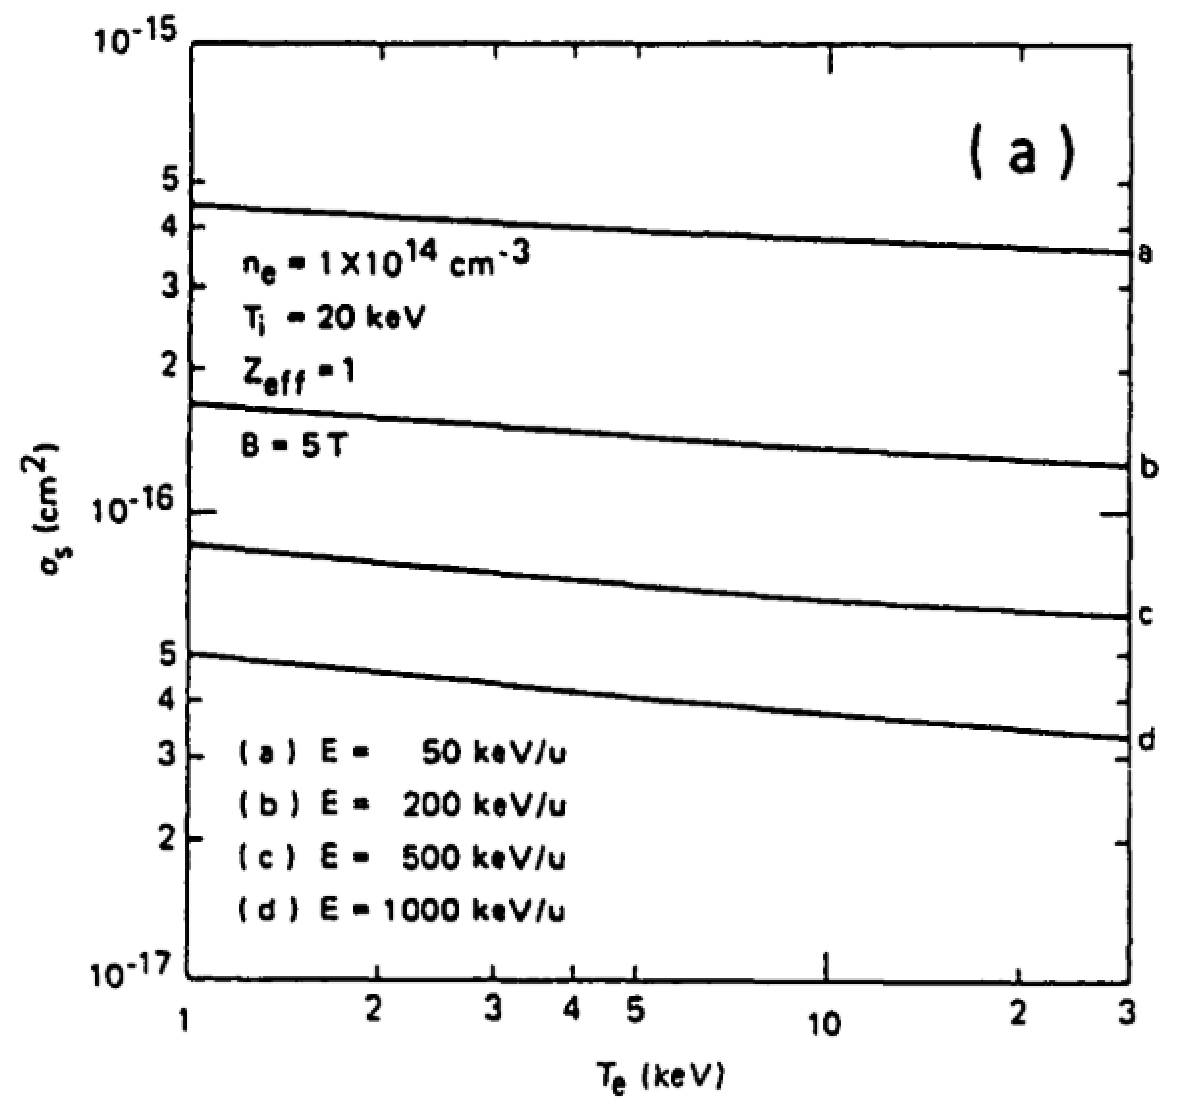
\includegraphics[width=0.45\linewidth]{images/beam_xsec_primary_temp_sweep}
		\label{fig:BeamXSecPrimaryTempSweep}
	} \quad
	\subfloat[$ Z_{eff} =2 $] {
		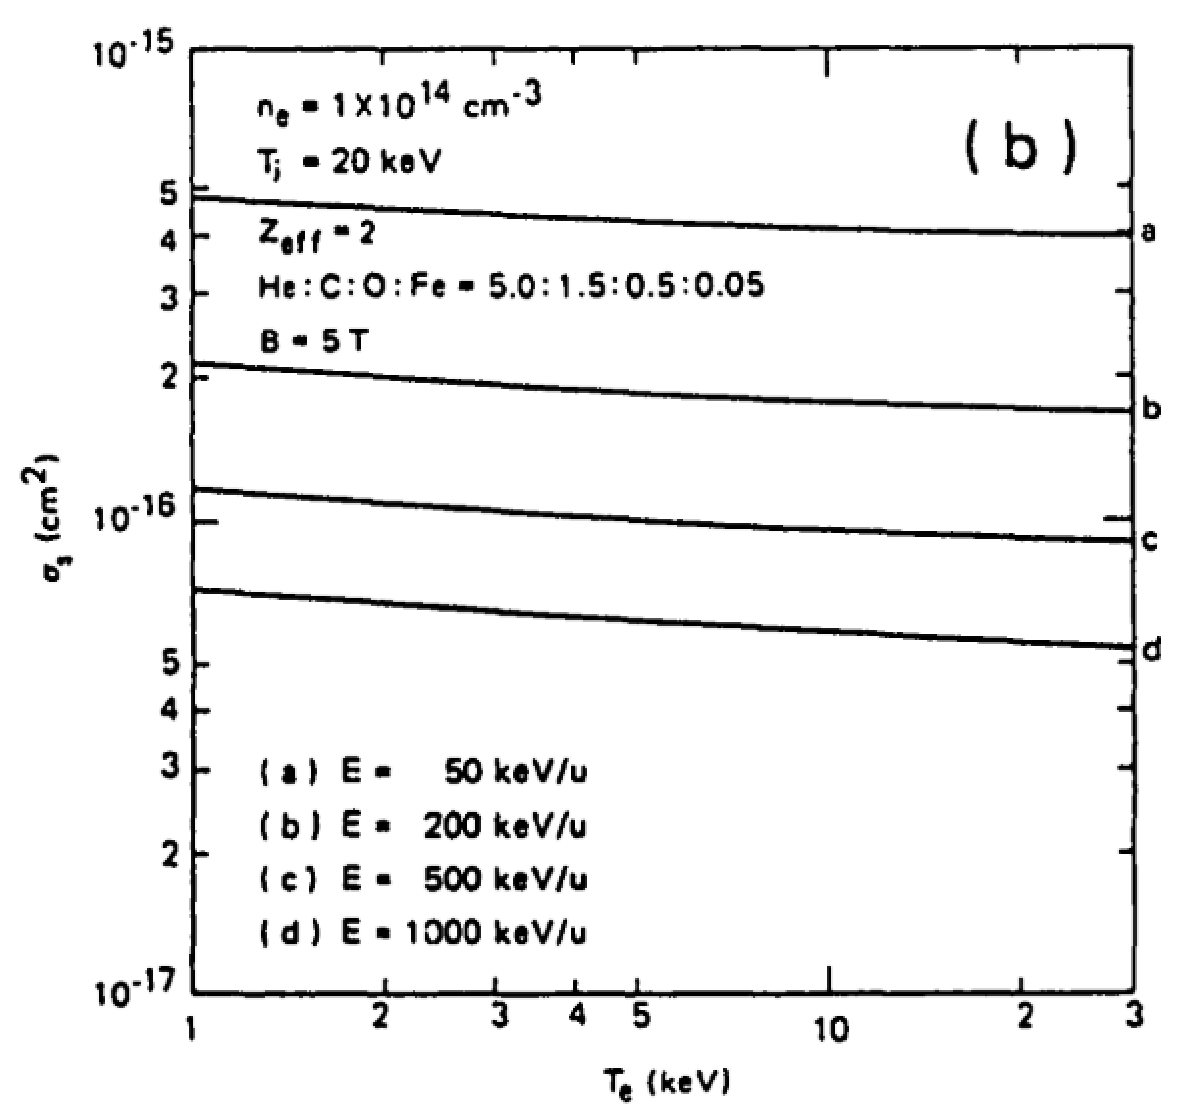
\includegraphics[width=0.45\linewidth]{images/beam_xsec_impurity_temp_sweep}
		\label{fig:BeamXSecImpurityTempSweep}
	}
	\caption{Temperature dependence of $\sigma_s$ for $n_e = 10^{14} \text{ cm}^{-3}$ for several beam energies \cite{Janev1989}}
\end{figure}


\begin{figure}[!ht]
	\subfloat[$ Z_{eff} = 1 $] {
		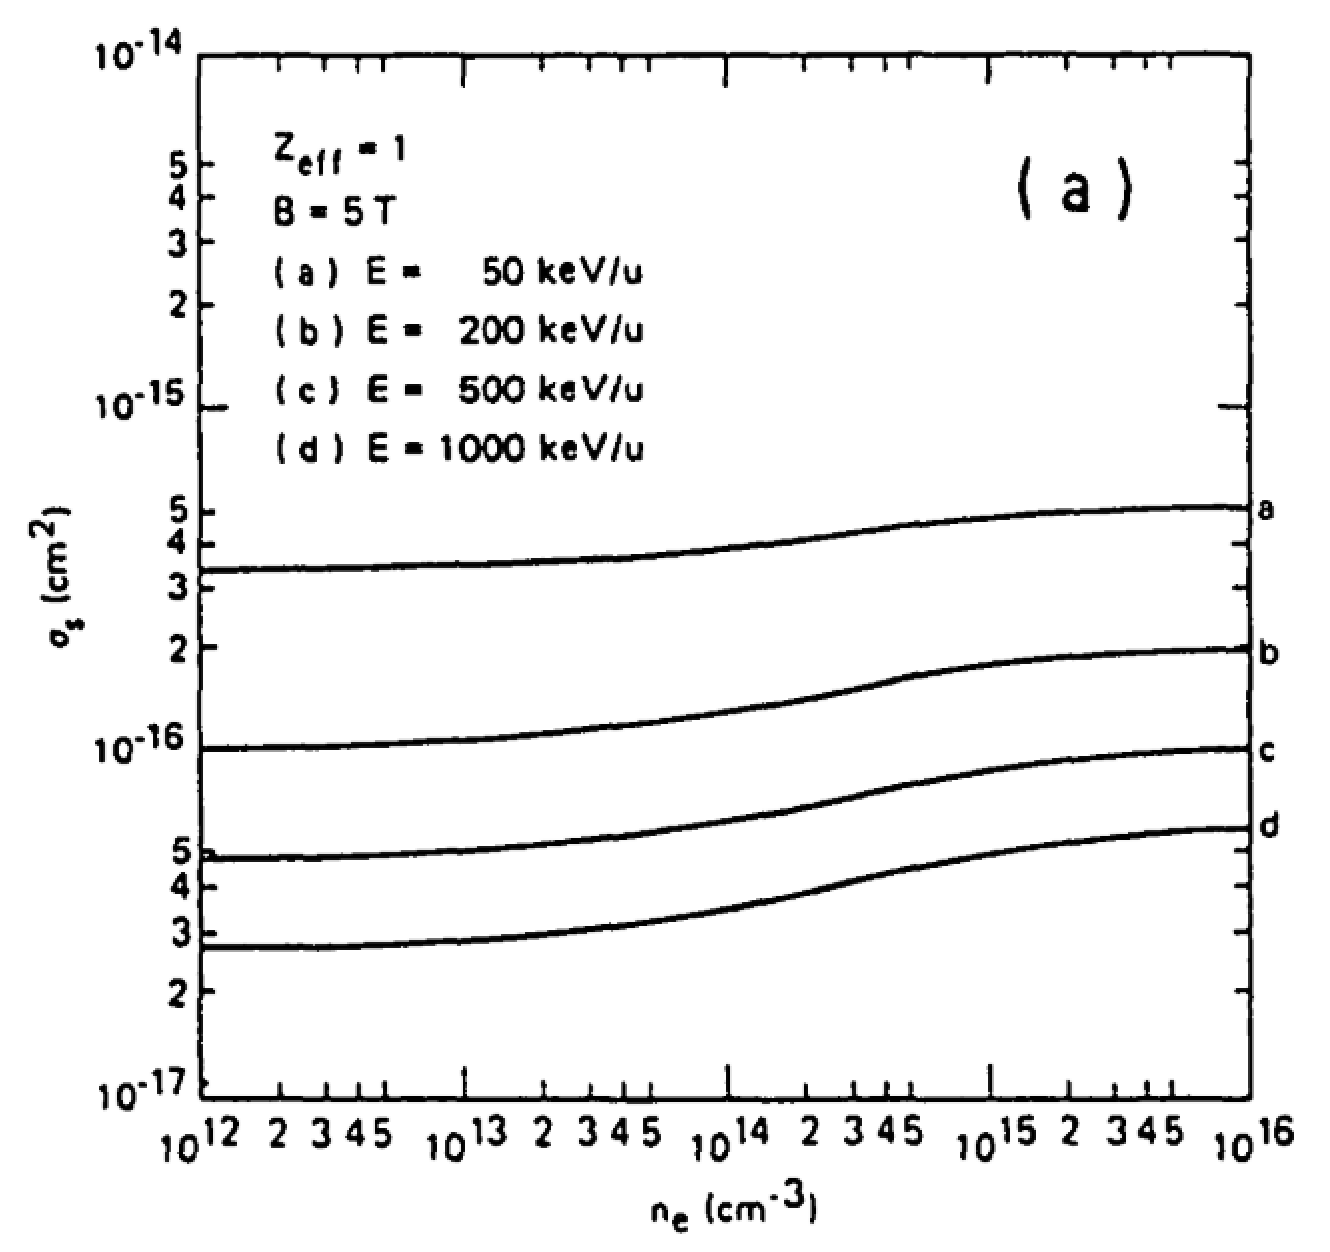
\includegraphics[width=0.45\linewidth]{images/beam_xsec_primary_den_sweep}
		\label{fig:BeamXSecPrimaryDenSweep}
	} \quad
	\subfloat[$ Z_{eff} =2 $] {
		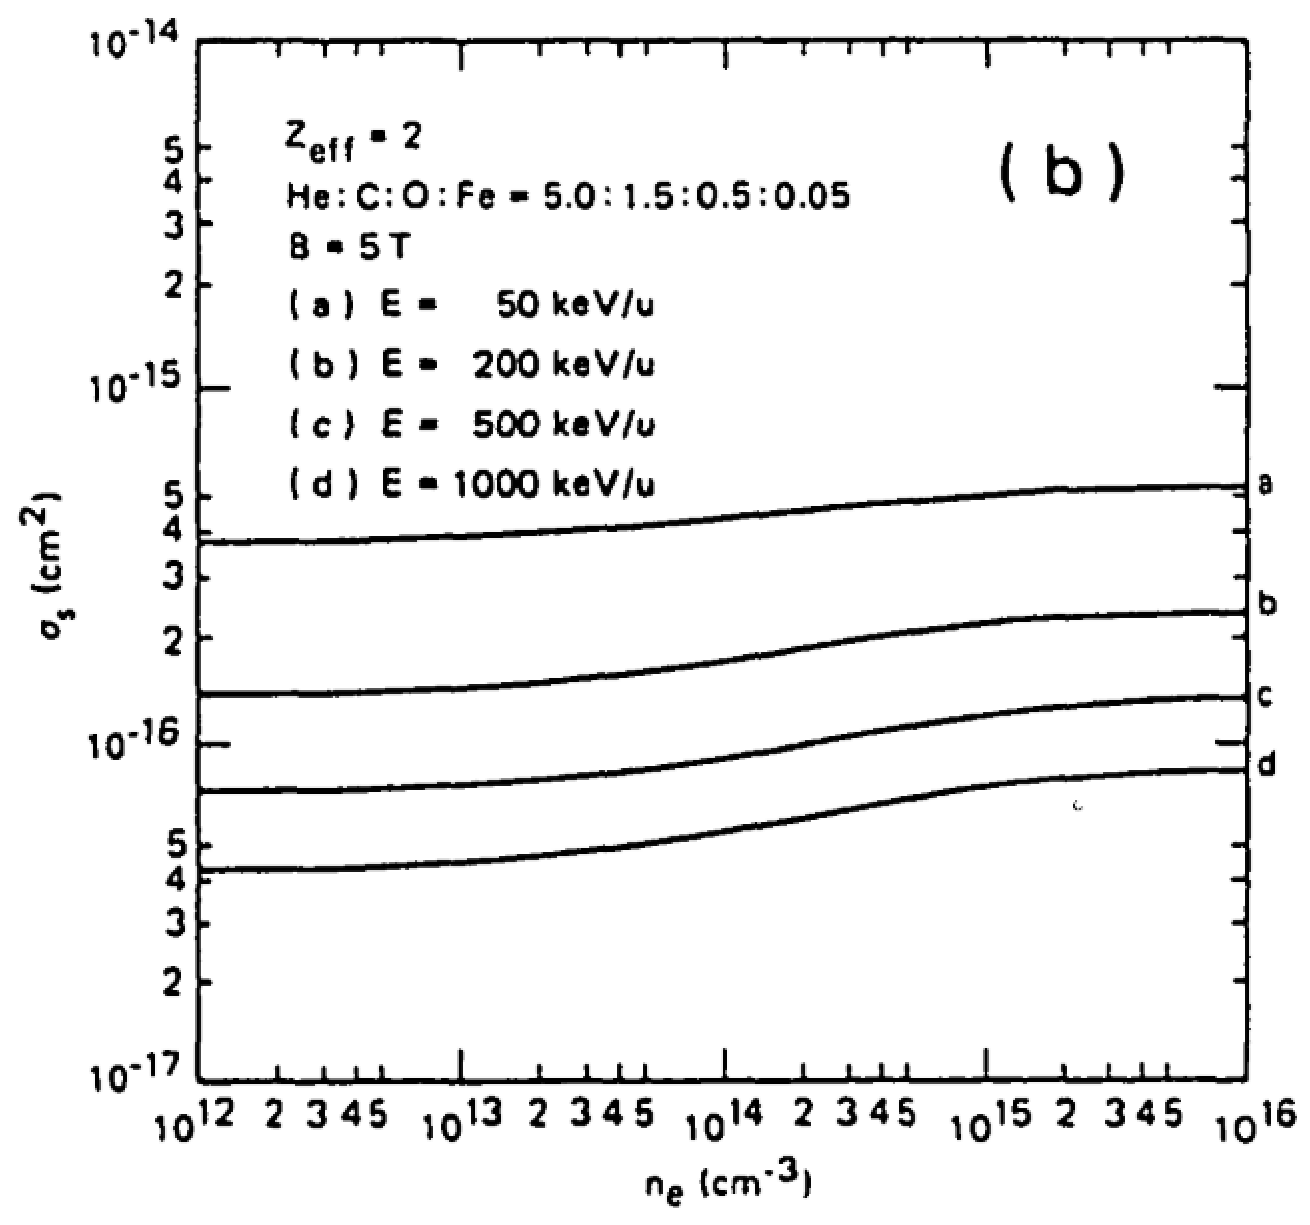
\includegraphics[width=0.45\linewidth]{images/beam_xsec_impurity_den_sweep}
		\label{fig:BeamXSecImpurityDenSweep}
	}
	\caption{Density dependence of $\sigma_s$ for several beam energies \cite{Janev1989}}
\end{figure}
%
%%\subsection{Ionization Modeling}\label{sub:Ionization}
%
%\subsection{Ideal Gas Law}\label{sub:IdealGasLaw}
%
%The relationship between the pressure calculated in the momentum equation and the density that initializes the iteration, there is an implied temperature which is given by the ideal gas law
%\begin{equation}
%	P = n\, T
%	\label{eqn:IdealGasLaw}
%\end{equation}
%Based on the iteration strategy chosen (\cref{sec:ComputationalModeling}), this temperature must align with the temperature implied by conservation of energy.
%
%\subsection{Pinch Diffusion} \label{sub:PinchDiffusion}

It is hoped that this research will culminate with an easy way to reincorporate the \vxb and \ac{IOL} physics into traditional diffusion models. In \cite{Stacey2019}, \citeauthor{Stacey2019} provides a diffusion-like model that has a $\Gamma^{Pinch}$ term that retains the \vxb and \ac{IOL}. $\Gamma^{Pinch}$, which appears in \cref{eqn:PinchDiffusion}, is given by the expression in \cref{eqn:PinchDiffusionFlux}.

\begin{equation}
	\diffp*{\left( D_{jj} \diffp{n_j}r \right)  }r - \diffp*{\left( D_{jk} \diffp{n_k}r \right)  }r - \diffp*{\left( D_{jj} \frac{n_j}{T_j}\diffp{T_j}r \right)  }r -\diffp*{\left( D_{jk} \frac{n_j}{T_k}\diffp{T_k}r \right)  }r + \diffp{\Gamma_{rj}^{pinch}}r = S_j
	\label{eqn:PinchDiffusion}
\end{equation}

\begin{equation}
	\Gamma_{rj}^{pinch} \equiv - \cfrac{n_j E_\phi^A}{B_\theta} - \cfrac{M_{\phi j}}{e_j B_\theta} + 
	\cfrac{n_j m_j \left( \nu_{jk} + \nu_{dj} \right) }{e_j B_\theta} 
	\left( \cfrac{E_r}{B_\theta} + \cfrac{B_\phi}{B_\theta} V_{\phi j} \right)
	- n_j m_j \nu_{jk} V_{\phi k}	
	\label{eqn:PinchDiffusionFlux}
\end{equation}
%
The diffusion coefficients embed the drag frequency, $\nu_{dj}$, and the inter-species collisional frequency $\nu_{jk}$.
%
\begin{equation}
		D_{jj} \equiv \cfrac{m_j T_j \left( \nu_{dj} + \nu_{jk} \right) }{\left(  e_j B_\theta \right)^2}, \quad
		D_{jk} \equiv \cfrac{m_j T_j \nu_{jk} }{ e_j e_k B_\theta^2}
		\label{eqn:PinchDiffusionCoefficients}
\end{equation}

%
%\subsection{Neutral Transport} \label{sub:NeutralTransport}

Neutrals from gas injection and gas recycling from the wall are:

\begin{itemize}
	\item ionized by interaction with electrons, which produces 
	\begin{itemize}
		\item a plasma ion in the ion particle balance equation \cref{eqn:Continuity} and
		\item an ionization cooling term in the ion energy balance equation \cref{eqn:EnergyIon}; and
	\end{itemize}
%
	\item interacts with a plasma ion to effectively replace a hot ion with a cool ion ( charge exchange cooling term in the ion energy balance equation \cref{eqn:EnergyIon}).
\end{itemize}

The transport of these neutrals are modeled using \acf{TEP} methodology \cite{Stacey1994, Stacey2000a, Stacey2001b, Rubilar2001, Stacey2001c, Mandrekas2003, Zhang2006}. The \ac{TEP} physics are based on a probabilistic description of interacting and transmitting particles within a region of interest (i). The partial current, $J_{ij}$ from a region i (note this is not indicating ions) to region j is described by \cref{eqn:GTneutPartialCurrent}.

\begin{equation}
	J_{ij} = \sum_{k}^{k}J_{ki}T_{0i}^{ku} + \sum_{k}^{i}\left(1-\sum_{l}^{i}T_{0i}^{kl}\right) J_{ki} c_i P_i \Lambda_{ij} + s_i P_i \Lambda{ij}^s
	\label{eqn:GTneutPartialCurrent}
\end{equation}

The first term accounts for all of the partial currents entering region i (see \prettyref{fig:tepschematic}) from all contiguous region k that transmit through region i. This is found by multiplying edge currents, $J_{ki}$ by the transmission probability $T_{0i}^{kj}$. The second term represents all of the partial currents entering region i from contiguous regions that suffer a collision inside of region i. The collision probability is $c_i$, the escape probability is, $P_i$ and the probability that scattered particles from region i escape to region j $\Lambda_{ij}$. The third term represents any internal source, such as recombination. Further description can be found in Section 2 of \citeauthor{Rubilar2001} \cite{Rubilar2001}.


\begin{figure}
	\centering
	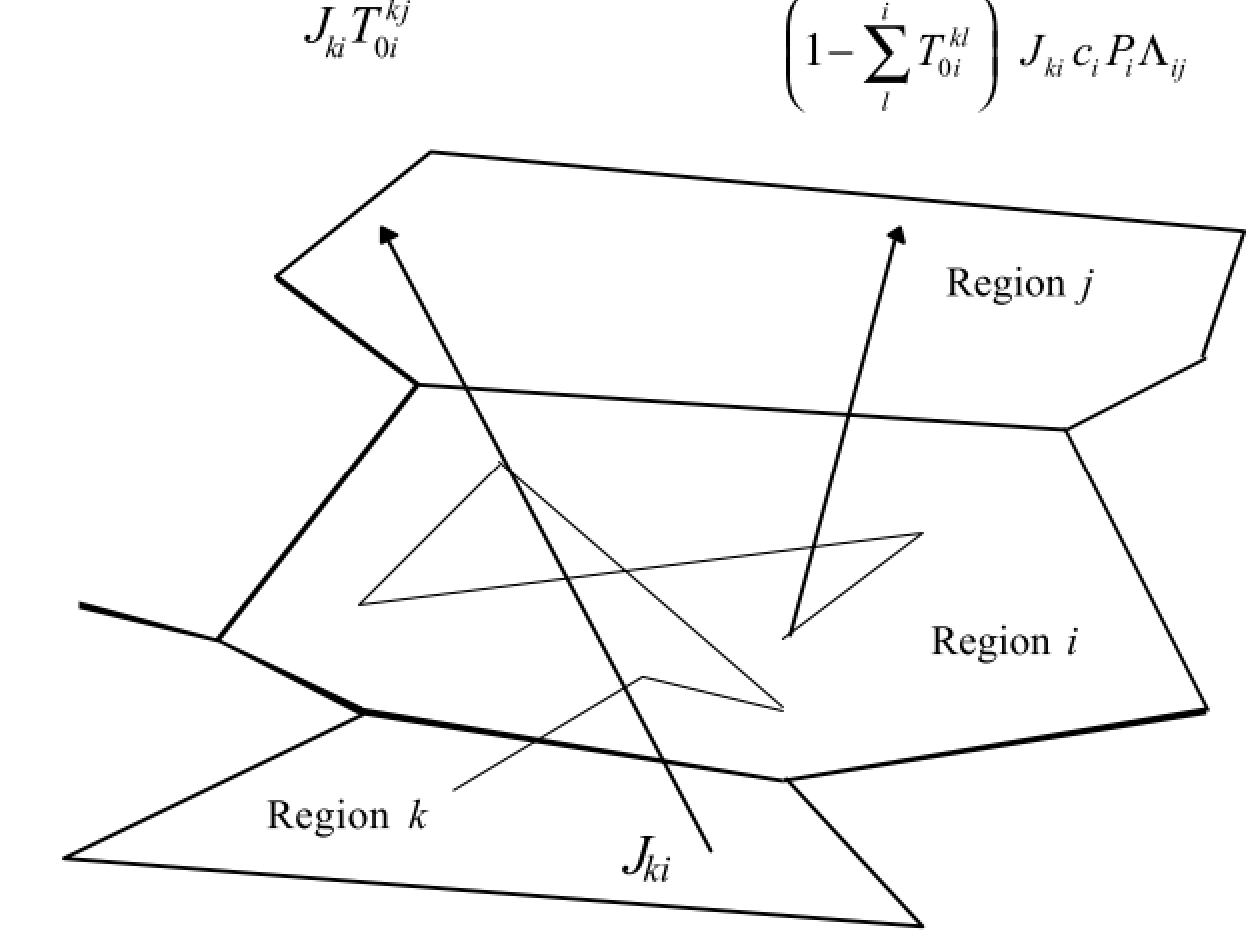
\includegraphics[width=0.7\linewidth]{images/TEP_schematic}
	\caption[TEP]{\acf{TEP} schematic diagram in 2-D geometry \cite{Rubilar2001}}
	\label{fig:tepschematic}
\end{figure}

For our purposes, it has been suggested that a simplified neutral transport implementation from \citeauthor{Stacey2000a} \citeyear{Stacey2000a} \cite{Stacey2000a}, utilizing GTNeut, should suffice. The simplified model breaks the plasma into regions shown in \prettyref{fig:gtneutschematic}. This modeling approach will be utilized initially and modified as needed.

\begin{figure}
	\centering
	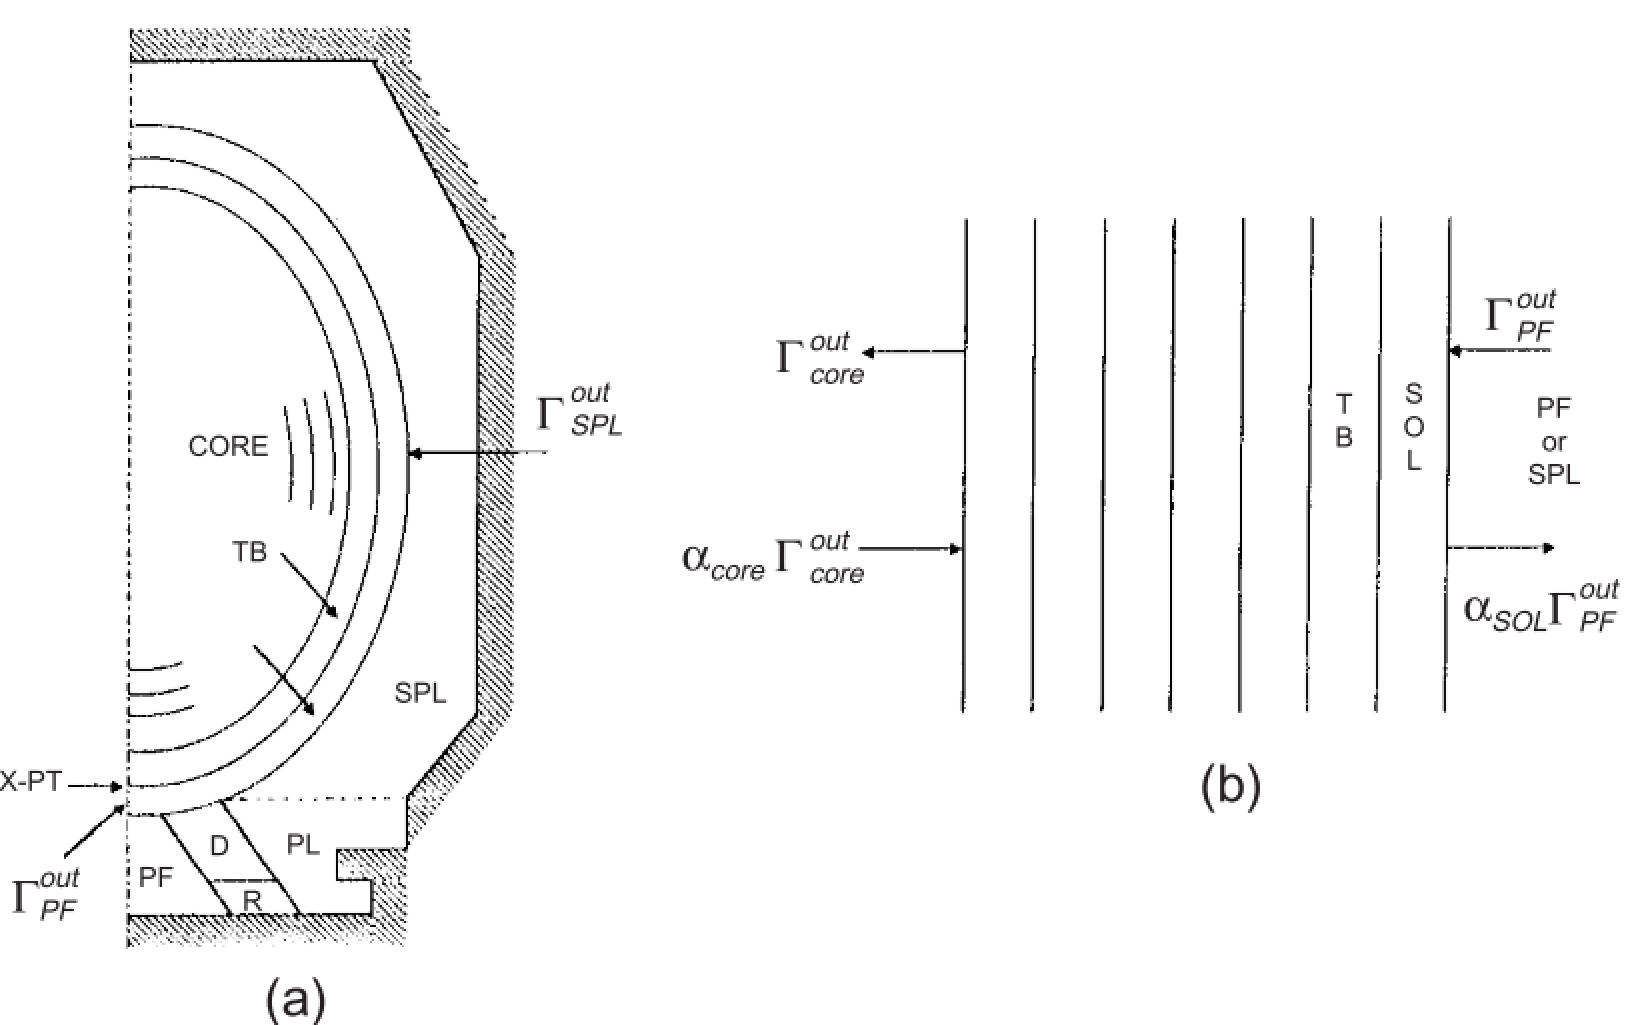
\includegraphics[width=0.7\linewidth]{images/GTNeut_schematic}
	\caption[GTNeutSchematic]{Schematic diagram of the neutral transport model: (a) 2-D TEP model of divertor plasma (D), recycling region (R), private flux (PF), plenum (PL) and SOL plenum (SPL); (b) 1-D ICB model of penetration through SOL and transport barrier (TB) into core. \cite{Stacey2000a}}
	\label{fig:gtneutschematic}
\end{figure}


